\chapter{Validación}

Para poner a prueba el sistema propuesto se desarrolló una breve prueba para obtener datos de usuarios reales y comprobar la efectividad del algoritmo a la hora de predecir preferencias. La prueba se realizó con alumnos de 4to año de Ingeniería Civil Informática, del ramo Ingeniería de Software. X personas participaron en esta prueba.

A continuación se explica el proceso utilizado para la obtención de datos.

\section{La aplicación de prueba.}

Para el caso de prueba se utilizaron 35 lugares turísticos, obtenidos desde el sitio ''Chile es Tuyo''  del Servicio Nacional del Turismo. \footnote{http://www.chileestuyo.cl/regiones/region-metropolitana/}. Para organizar los lugares se utilizaron marcadores para clasificarlos según la naturaleza del destino turístico. Por ejemplo, los lugares de esquí y cercanos a la cordillera se clasificaron como ''Nieve''. Los lugares ubicados dentro de la ciudad de Santiago se consideraron ''Urbanos''. Así mismo para ''Rural'', ''Aire Libre'' y ''Artístico''. (adjuntar tabla con clasificacion de cada lugar).

A cada usuario se le asignaron 10 lugares de forma semi-aleatoria, ya que se consideran 2 ítems de cada categoría (2 Lugares de Nieve, 2 Urbanos, 2 Rurales, 2 de Aire Libre y 2 Artísticos.). Una vez seleccionados son desplegados al alumno de la siguiente forma.

\begin{figure}[hbtp]
\centering
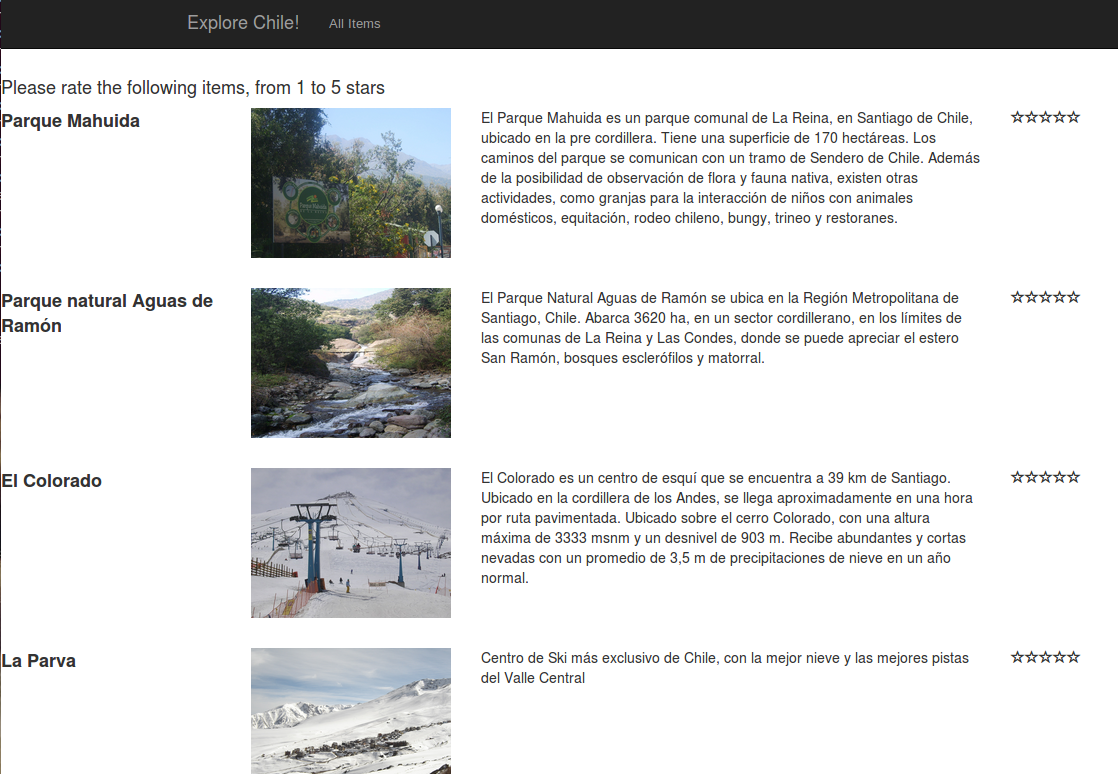
\includegraphics[scale=0.65]{images/rate.png}
\caption{Vista de calificación para cada prueba}
\end{figure} 

En esta vista el alumno debía calificar cada lugar usando las estrellas de la derecha, con un puntaje que considera la escala del 1 al 5 (Explicar por qué se usó la escala del 1 al 5).

Cuando todos los alumnos hayan terminado de calificar, aquellos que hayan recibido más de dos lugares recomendados pasaron a la siguiente etapa.

\begin{figure}[hbtp]
\centering
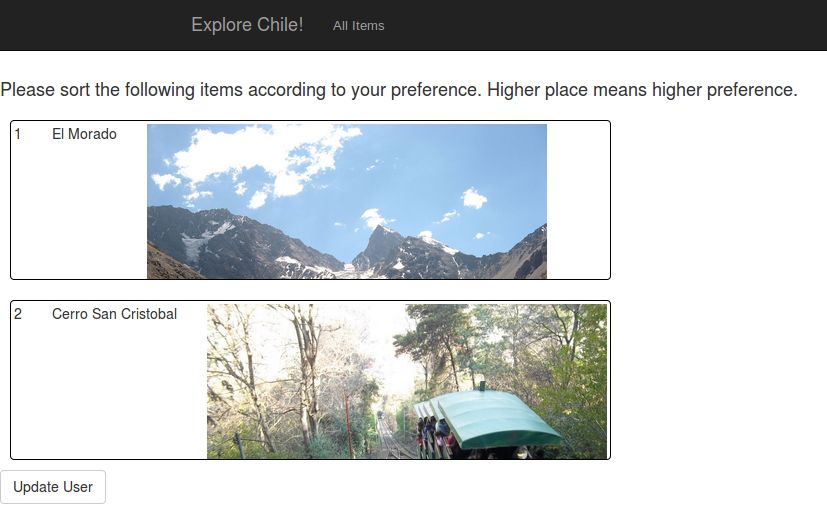
\includegraphics[scale=0.75]{images/sort.png}
\caption{Vista de ordenamiento para cada prueba}
\end{figure}  

En esta etapa el alumno debe arrastrar los ítems en pantalla, desde el de mayor interés al de menor. (Arriba hacia abajo). De esta forma se puede obtener una declaración explícita de la satisfacción del usuario respecto a los ítems que se consideran relevantes.

\section{Resultados}

\section{Análisis de resultados}

(Incluir comparación de ranking predicho y ranking real para cada almuno.)

